%%%% Proceedings format for most of ACM conferences (with the exceptions listed below) and all ICPS volumes.


%\documentclass[sigconf]{acmart}
%%%% As of March 2017, [siggraph] is no longer used. Please use sigconf (above) for SIGGRAPH conferences.

\documentclass[manuscript]{acmart}

\usepackage{url}
%\usepackage[round]{natbib}
%\usepackage[natbib, style=authoryear, backend=bibtex]{biblatex}
\usepackage{tikz}
\usetikzlibrary{mindmap}

%%%% Proceedings format for SIGPLAN conferences 
% \documentclass[sigplan, anonymous, review]{acmart}

%%%% Proceedings format for SIGCHI conferences
% \documentclass[sigchi, review]{acmart}

%%%% To use the SIGCHI extended abstract template, please visit
% https://www.overleaf.com/read/zzzfqvkmrfzn

%
% defining the \BibTeX command - from Oren Patashnik's original BibTeX documentation.
%\def\BibTeX{{\rm B\kern-.05em{\sc i\kern-.025em b}\kern-.08emT\kern-.1667em\lower.7ex\hbox{E}\kern-.125emX}}

\usepackage{booktabs} % For formal tables
%\usepackage{inputenc}
\usepackage[utf8]{inputenc}
\usepackage{dblfloatfix}
\usepackage{tabularx}
\newcolumntype{L}{>{\raggedright\arraybackslash}X}
\usepackage{xcolor}% Add more colours
\usepackage{fancybox}%Provides variants of \fbox
\usepackage{balance}


%%%%%%%%%%%%%%%%%%%%%%%%%%%%%%%%%%%%%%%%%%%%%
%%%% -- Conditional compilation settings
\usepackage{ifthen}
\newboolean{includecomments}
\setboolean{includecomments}{true}
%%%% --- End of conditional compilation settings
%%%%%%%%%%%%%%%%%%%%%%%%%%%%%%%%%%%%%%%%%%%%%

%\usepackage{amssymb} %adds special symbol names used for \TOFIX commands etc
\usepackage{xcolor}
\usepackage{hhline}
%\nb - keyword - color - comment
\ifthenelse{\boolean{includecomments}} {
    \newcommand{\nb}[3]{
    	{\colorbox{#2}{\bfseries\sffamily\scriptsize\textcolor{white}{#1}}}
    	{\textcolor{#2}{\sf\small$\blacktriangleright$\textit{#3}$\blacktriangleleft$}}}
} {
    \newcommand{\nb}[3]{}
}

\newcommand{\serge}[1]{\nb{Serge: }{blue}{[#1]}}
\newcommand{\mercy}[1]{\nb{Mercy: }{purple}{[#1]}}
\newcommand{\todo}[1]{\nb{TODO: }{orange}{[#1]}}
\newcommand{\tofix}[1]{\nb{TO FIX:}{red}{[#1]}}

\newcommand{\hypobox}[1]{
	\begin{center}%
        \noindent\thicklines\setlength{\fboxsep}{2pt}%
        \cornersize{0.1}
        \ovalbox{\begin{minipage}{8.4cm}%
		#1
		\end{minipage}}
	\end{center}}
    
% Rights management information. 
% This information is sent to you when you complete the rights form.
% These commands have SAMPLE values in them; it is your responsibility as an author to replace
% the commands and values with those provided to you when you complete the rights form.
%
% These commands are for a PROCEEDINGS abstract or paper.


%
% These commands are for a JOURNAL article.
%\setcopyright{acmcopyright}
%\acmJournal{TOG}
%\acmYear{2018}\acmVolume{37}\acmNumber{4}\acmArticle{111}\acmMonth{8}
%\acmDOI{10.1145/1122445.1122456}

%
% Submission ID. 
% Use this when submitting an article to a sponsored event. You'll receive a unique submission ID from the organizers
% of the event, and this ID should be used as the parameter to this command.
%\acmSubmissionID{123-A56-BU3}

%
% The majority of ACM publications use numbered citations and references. If you are preparing content for an event
% sponsored by ACM SIGGRAPH, you must use the "author year" style of citations and references. Uncommenting
% the next command will enable that style.
%\citestyle{acmauthoryear}

%
% end of the preamble, start of the body of the document source.
\begin{document}

%
% The "title" command has an optional parameter, allowing the author to define a "short title" to be used in page headers.
%\title{Balancing Speed vs Quality - A Multivocal Literature Review on Technical Debt Management in Startups}
\title{Balancing Speed vs Quality - A Multi-vocal Literature Review on Technical Debt in Startups}
%
% The "author" command and its associated commands are used to define the authors and their affiliations.
% Of note is the shared affiliation of the first two authors, and the "authornote" and "authornotemark" commands
% used to denote shared contribution to the research.
\author{Mercy Njima}
\orcid{1234-5678-9012-3456}
\affiliation{
	\institution{University of Antwerp and Flanders Make}
	%\streetaddress{104 Jamestown Rd}
	\city{Antwerp}
	%\state{VA}
	%\postcode{23185}
	\country{Belgium}}
\email{mercy.njima@uantwerpen.be}

\author{Serge Demeyer}
\orcid{1234-5678-9012-3456}
\affiliation{
	\institution{University of Antwerp and Flanders Make}
	%\streetaddress{104 Jamestown Rd}
	\city{Antwerp}
	%\state{VA}
	%\postcode{23185}
	\country{Belgium}}
\email{serge.demeyer@uantwerpen.be}

%
% By default, the full list of authors will be used in the page headers. Often, this list is too long, and will overlap
% other information printed in the page headers. This command allows the author to define a more concise list
% of authors' names for this purpose.
%\renewcommand{\shortauthors}{M. Njima, S. Demeyer}

%
% The abstract is a short summary of the work to be presented in the article.
\begin{abstract}
 Startups often operate under limited resources and time, and may intentionally accumulate technical debt to meet immediate market needs.
 However, this intentional accumulation requires careful management to avoid long-term negative consequences for the startup.
 We conducted a Multivocal Literature Review of the existing body of knowledge in order to understand the state of the art and the practice
 of technical debt in startups and its implications. The key outcome of this study is the creation of a framework that provides a
 comprehensive view of technical debt in startups including it's dimensions and attributes as well as a taxonomy that describes the
 different forms it takes and directions for future work.
\end{abstract}
%
% The code below is generated by the tool at http://dl.acm.org/ccs.cfm.
% Please copy and paste the code instead of the example below.
%

\maketitle

\section{Introduction}
In software development, technical debt is a term that is used to describe the compromises that allow a team to deliver a project quickly at the cost of increased maintenance in the future ~\cite{Maldonado7332619}. These compromises create software "debt" that must be repaid in the future to  avoid "interest" in the form of reduced maintainability and evolution ~\cite{Seaman6225999}. Most research on technical debt has been focused on mature software teams say in large organizations who may have less pressure and, therefore, reason about technical debt very differently than software startups ~\cite{Besker2018,Li:2015}. However, technical debt is a common challenge for startups, as they often prioritize rapid development over long-term maintainability. While taking on technical debt can help startups get to market faster, it can also lead to increased development costs, decreased quality, and hindered innovation over time ~\cite{Seaman6225999, DesignSt86:online}.

\subsection{Significance of Technical Debt in Startup Environments}
Startups are organizations that create scalable, high-tech innovative products and services under conditions of extreme uncertainty, limited resources, multiple influences, new technologies, and evolving markets~\cite{Unterkalmsteiner16,Sutton854066}. Startups often operate under resource constraints and time pressure, have inexperienced developers, lack a defined development process, and lack autonomy of decision-making, which lead to the intentional or unintentional accumulation of technical debt ~\cite{Besker2018}. Klotins et al. explored technical debt in start-ups and found that excessive technical debt could be a cause for missed market opportunities and contribute to start-up failures ~\cite{Klotins:2018:ETD}. The situation is further exacerbated by the need for rapid product development and iteration to gain a competitive advantage in the market ~\cite{Cico0JNM20}.

\subsection{Purpose and Scope of Review}
While technical debt is as important to software startups as it is to mature companies, the kind of decisions to be made and the consequences of making the wrong decisions are not the same, justifying further research on technical debt in software startups ~\cite{Unterkalmsteiner16}. Studies have demonstrated that startups tend to accumulate more technical debt compared to established companies due to their relentless pursuit of faster time to market and product launches. This inherent pressure often leads to the adoption of shortcuts, quick fixes, and less maintainable code structures, which can manifest in various negative consequences ~\cite{Giardino2016,Klotins882019}. In the recent past, there has been a few research efforts to investigate the technical debt phenomenon in startups. However, no structured investigation of the area has been performed and none of the systematic literature reviews or mapping studies on technical debt address technical debt in startups. The goal of this work is to identify and understand the main contributions of the state-of-art and practice of technical debt in startups. Given the industry-oriented nature of startups and the limited number of formally-published literature in this area, we conducted a Multivocal Literature Review (MLR) ~\cite{GAROUSI2019101}. We chose this method because a significant amount of information related to the research topic is available in grey literature, including technical reports, blogs, and standards that are not typically published in academic sources. MLRs recognize the need for grey literature rather than constructing evidence from only the knowledge reported in academic settings.
This work was conducted with the goal of answering the following research questions:
\begin{enumerate}
\item What is the current state-of-the-art research and practice of technical debt in startups?
\item {What factors influence the accumulation of technical debt in software startups?}
%\item {What are the challenges and benefits of technical debt for software startups?}
\item {How do startups manage technical debt and when does that become a priority?}
\item What are the reported mitigating strategies of technical debt in startups?
\item What are the possible future directions of technical debt research and practice in startups?
\end{enumerate}

The rest of this paper is structured as follows: Section \ref{Sec:Research} presents the design and method of this work. Section \ref{Sec:Results} discusses the findings and Section \ref{Sec:Discussion} presents a discussion of the findings and answers our research questions. We present the conclusion and examine threats to validity in Section \ref{Sec:Threats}. Finally, Section \ref{Sec:Conclusion} presents the conclusion and future work.

\section{Research Design}\label{Sec:Research}
Various approaches for conducting literature reviews are available such as systematic mapping studies, systematic literature reviews, snowballing, and multi-vocal literature reviews. In the software engineering field, many researchers frequently perform systematic literature reviews and mapping studies. These approaches are typically employed when a sufficient number of academic peer-reviewed articles on a particular subject are accessible. During our preliminary study, we identified a limited quantity of peer-reviewed articles on our topic. One reason for this scarcity of peer-reviewed literature could be that startup technical debt is quite new research topic. Therefore, we had to explore other sources of literature, often referred to as multi-vocal literature. Multi-vocal literature include gray literature such as blog posts, web articles, trade journal articles, and white papers. In conducting a multi-vocal literature review, (MLR) we aim to provide a comprehensive and inclusive understanding of technical debt in startups by incorporating a wide range of sources and perspectives from both peer-reviewed and non-published literature ~\cite{Ogawa91, Garousi2016/2915970.2916008}. This approach is particularly valuable in software engineering in startups, where it is essential to capture both the "state of the practice" and " state of the art/research" and therefore, provide a more holistic view of the field. 

The MLR process is illustrated in Fig. \ref{fig:MLRprocess}. We followed the established procedures and guidelines defined by Garousi et al. ~\cite{GAROUSI2019101}. It consists of three phases: planning, conducting and reporting. We discuss each phase in the rest of this section. This MLR search was conducted in October 2023 and the analysis and reporting was completed in December 2023.

\begin{figure}
  \includegraphics[width=\textwidth]{MLRprocess.jpg}
  \caption{Multi-vocal literature review (MLR) process adopted in this research ~\cite{SALTAN2021106510}}
  \Description{}
 \label{fig:MLRprocess}
\end{figure}

\subsection{Conducting the MLR}
The MLR search was conducted in three stages.
\begin{enumerate}
\item Data sources and search strategy: For the formal literature, we selected the list of relevant bibliographic sources following the suggestions of ~\cite{kitchenham2007guidelines}, since these sources are
recognized as the most representative in the software engineering domain. The list is: 
\begin{enumerate}
   \item ACM Digital Library
\item IEEEXplore Digital Library
\item Science Direct
\item Scopus
\item CiteSeer library
\item Inspec
\item Springer link
\end{enumerate} 

Thereafter, we applied the snowballing method in order not to miss any potentially relevant publications as outlined in ~\cite{Wohlin2014/2601248.2601268}.
On the other hand, we used Google's web search engine (http://www.google.com) to source for the grey literature.
A preliminary search helped to narrow down the keywords for a suitable search query. We used the terms "technical debt" AND "startup" for both the formal and the grey literature searches.

\item Inclusion and exclusion criteria: The results were reviewed against a set of inclusion and exclusion criteria. Search results were included if 
\begin{enumerate}
\item the main objective of the result which may be a primary or secondary  study was either to discuss or investigate technical debt in startups. This inclusion criterion defines the basic scope of our study.
\item must have a software engineering context. To keep our study to manageable levels, the scope of our study was restricted to SE related papers.
\end{enumerate}
Search results were excluded if they were 
\begin{enumerate}
\item sources not in English
\item a duplicated record 
\item only mention technical debt in an introductory manner and do not fully or partly focus on its occurrence in startup context.
\end{enumerate}
\item Quality assessment: To apply quality assessment criteria, we adopted the 11-factor quality
assessment criteria proposed by Dybå et al. ~\cite{DYBA2008833} for scientific literature. We adopted the quality assessment checklist of grey literature from Garousi et al. ~\cite{GAROUSI2019101}.
Each criterion was graded on a binary (‘1’ or ‘0’) grade. This technique helps to limit the degree of subjectivity and report the results more objectively. 
\end{enumerate}

\section{Findings}\label{Sec:Results}
In this section, we present the results from analysing 70 primary sources. The results begin with the demographic information which tells us the type of literature, type of sources and publication trend over the years. We will then present a detailed assessment based on the thematic analysis.

\subsection{Demographics}
%Classification / types of literature
A growing body of research has shed light on the intricacies of technical debt in startups. Figure \ref{fig:Trend} presents the publication trend over that years and shows that there's been active and growing research efforts evident since 2019.


\begin{figure}
%  \includegraphics[width=\textwidth]{PublicationTrend.jpg}
  \caption{Publication Trend over the years}
  %\Description{}
 \label{fig:Trend}
\end{figure}

Figure \ref{fig:Sources} shows the categories of our primary sources. The highest number of resources we cited came from web blogs and the second highest number of resources were presented at conferences. This clearly shows high practitioners’ interest in the topic under study. 

\begin{figure}
%  \includegraphics[width=\textwidth]{TypeSources.jpg}
  \caption{Types of Primary Sources}
  %\Description{}
 \label{fig:Sources}
\end{figure}

\subsection{State of the art}
In this section, we discuss different types of technical debt accrued by startups with the help of relevant examples. This section answers RQ1 - What is the current state-of-the-art research and practice of technical debt in startups?

\subsection{Key Dimensions and Types of Technical Debt}
The main dimensions of technical debt that start-ups struggle with are:

\subsubsection{Code Debt} 
Code debt is a major concern for startups. It refers to the accumulation of sub-optimal or inefficient code within a startup's software code base . Poorly written code, novice coding and sub-optimal code impacts quality due to complex logic, code clones, and bad coding style . Poorly structured and documented code, known as code smells, have the most severe impact on both productivity and quality in start-ups ~\cite{Klotins2018/3183519.3183539}

This can occur due to various reasons such as time constraints, resource limitations, evolving requirements, or inexperienced developers. Code debt is a form of technical debt that can negatively impact a startup's ability to scale, innovate, and maintain its software product over time ~\cite{FowlerBottlenecks, Qualityv77:online}.

Startups can address code debt by having regular code reviews, refactoring sessions, investment in developer education and training, and fostering a culture of quality and craftsmanship ~\cite{10043622, Acknowle63:online}.

\subsubsection{Testing Debt}
Testing is a crucial aspect of software development, but in the fast-paced world of startups, it's easy to accumulate testing debt. This refers to the shortcuts taken in testing practices, leading to a backlog of untested functionalities or inadequate test coverage  ~\cite{Howtohan98:online}. This may be due to limited test coverage where startups might focus on core functionalities at launch, leaving peripheral features with minimal or no testing. This can lead to bugs and stability issues down the line ~\cite{Totalqua26:online}.

Implementing automated testing frameworks, such as unit tests, integration tests, and regression tests, helps maintain the stability and reliability of the application. By establishing a robust test suite, startups can catch potential issues before they impact the user experience and prevent the accumulation of technical debt ~\cite{TheImpac54:online}. Reliance on manual testing can be time-consuming and error-prone, especially as the code base grows ~\cite{Howtohan98:online}.

Managing testing debt is an ongoing process. By prioritizing testing practices, adopting automation, and continuously improving the test suite, startups can ensure their product remains stable and high-quality as it evolves ~\cite{CrowneWhyStartupsFail, 1NewMess49:online}.

\subsubsection{Architecture Debt}
Architecture debt, refers to the accumulation of sub-optimal design choices that create technical limitations and increase development complexity as the product scales ~\cite{Startups4:online}. The initial architecture may not be designed to handle an increase in users or data volume. This can lead to performance issues and system outages as the startup scales ~\cite{Qualityv77:online}.

Startups often begin with a monolith, a single code base handling all functionalities. While this is efficient initially, it can become a bottleneck for scalability and maintenance as the product grows. Startups should consider breaking down the single base into smaller, independent services that communicate with each other. This will improve scalability, maintainability, and deployment flexibility ~\cite{Howtohan98:online, DesignSt86:online}

\subsubsection{Documentation Debt}
Documentation debt refers to the lack of clear, concise, and up-to-date documentation for a product's code base, processes, and functionalities. When code lacks proper documentation, developers waste time deciphering its functionality and purpose. This slows down development and increases the risk of errors ~\cite{The3Best94:online, 10.1145/3493244.3493254}.

Moreover, troubleshooting issues or fixing bugs becomes more difficult without proper documentation. Developers might need to rely on tribal knowledge or reverse-engineer the code, increasing maintenance costs ~\cite{DesignSt86:online}.

\subsubsection{People Debt}
People Debt refers to the negative consequences of neglecting employee well-being, knowledge transfer, and building a strong company culture in the early stages of a startup ~\cite{Blog21:online}. 


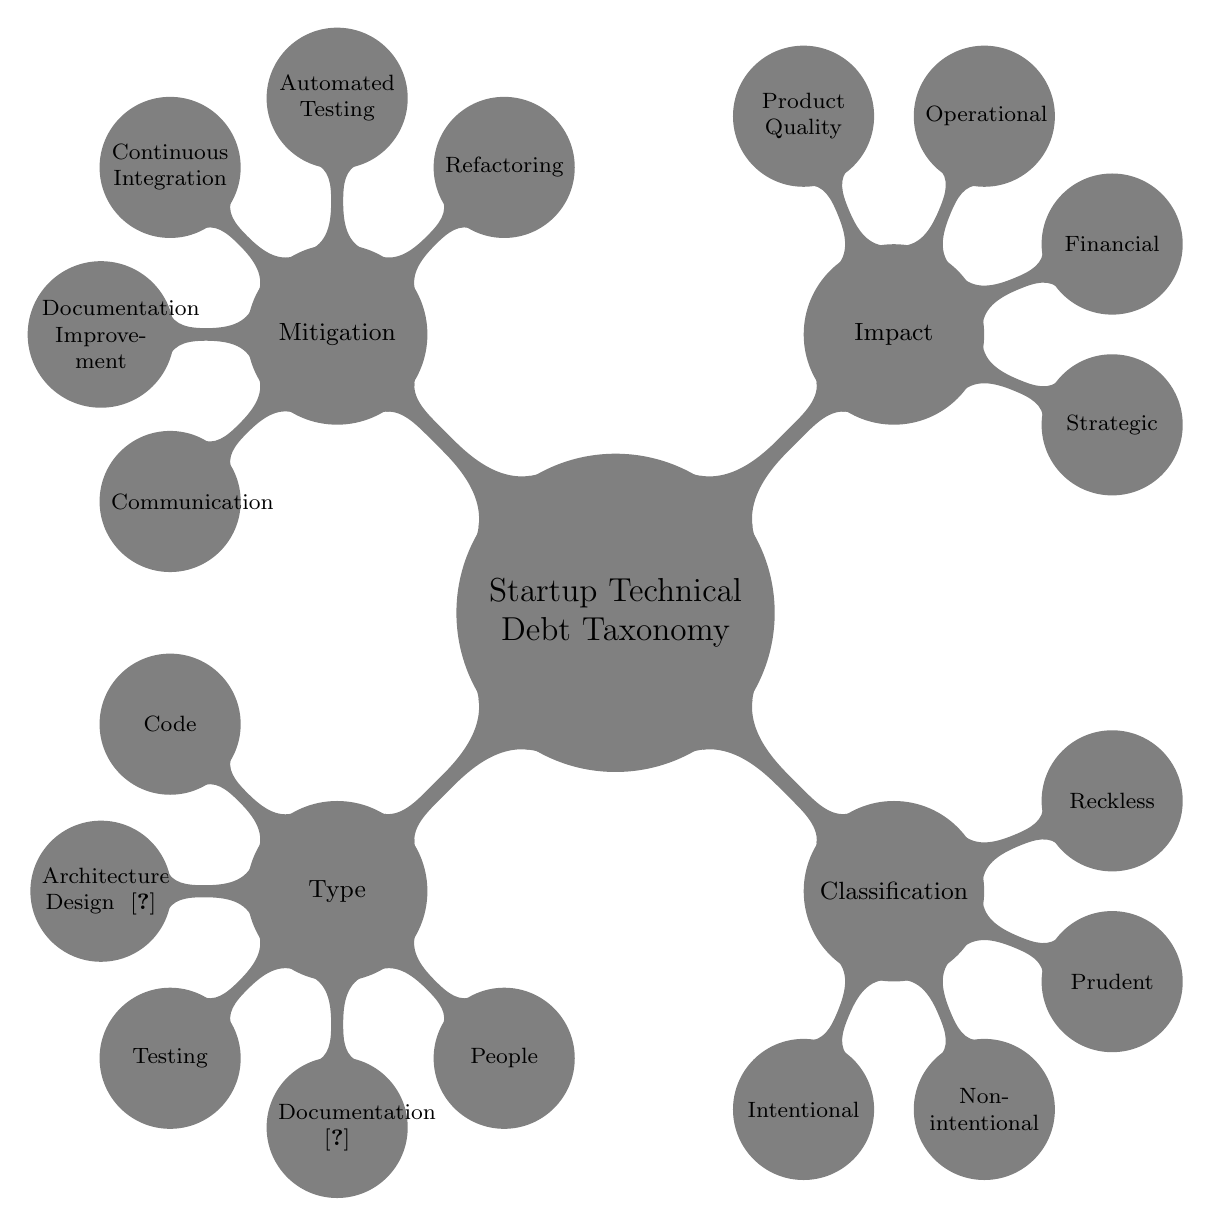
\begin{tikzpicture}[mindmap, grow cyclic, every node/.style=concept, concept color=gray, 
	level 1/.append style={level distance=5cm,sibling angle=90},
	level 2/.append style={level distance=3cm,sibling angle=45},]

\node{Startup Technical Debt Taxonomy}
child [concept color=gray] {node {Type}
	child { node {Code}}
	child { node {Architecture, Design ~\cite{Qualityv77:online}}}
	%child { node {Infrastructure}}
	child { node {Testing}}
	child { node {Documentation ~\cite{GAROUSI2019101}}}
	child { node {People}}
	%child { node {}}
}
child [concept color=gray] { node {Classification}
	child { node {Intentional}}
	child { node {Non-intentional}}
	child { node {Prudent}}
	child { node {Reckless}}
	%child { node {}}
}
child [concept color=gray] { node {Impact}
	child { node {Strategic}}
	child { node {Financial}}
	child { node {Operational}}
	child { node {Product Quality}}
	%child { node {}}
}
child [concept color=gray] { node {Mitigation}
	child { node {Refactoring}}
	child { node {Automated Testing}}
	child { node {Continuous Integration}}
	child { node {Documentation Improvement}}
	child { node {Communication}}
};

\end{tikzpicture}

\subsection{Technical Debt Accumulation Causes}
Technical debt accumulation in startups can be attributed to various factors. Besker et al. found that the intentional accumulation of technical debt in startups is influenced by organizational factors such as the startup phase, developers' experience, founders' software knowledge, and employee growth ~\cite{Besker2018}. Additionally, Klotins et al. highlighted that prioritizing development speed over quality, team aspects, and lack of resources contribute to the accumulation of technical debt in startups ~\cite{Klotins:2018:ETD}. Furthermore, they emphasized the trade-off between development speed and accumulated technical debt as a crucial determinant for the success of early-stage startups.

Unwanted technical debt in startups can arise due to poor engineering decisions, sloppy individual attitudes, and insufficient coordination of engineering work ~\cite{Klotins882019}. The study emphasized the need to model the evolutionary nature of technical debt accumulation, considering the interplay between its benefits and costs over the software product's life cycle.

Technical debt in startups can accumulate due to a variety of factors, including:
\subsubsection{Pressure to meet deadlines and product milestones}
Startups often face intense pressure to launch their products quickly and meet market demands. This can lead to the prioritization of rapid development over long-term maintainability, encouraging the use of shortcuts, quick fixes, and less maintainable code structures ~\cite{Klotins:2018:ETD,Qualityv77:online}. In addition, there's also shorter development cycles. Rapid iteration cycles and frequent feature releases leave little time for code refactoring or comprehensive testing, potentially introducing bugs and inefficiencies.

\subsubsection{Limited resources and tight budgets}
Startups typically operate with limited resources and budgets, making it challenging to invest in comprehensive planning, thorough testing, and robust architectural design. This can contribute to the accumulation of technical debt, as developers may opt for expediency over quality ~\cite{FowlerBottlenecks,Balancin62:online}. Furthermore, early-stage startups often have small development teams with limited technical expertise. This can make it difficult to invest time in writing clean code, thorough documentation, and robust tests.

\subsubsection{Changing requirements and scope}
Startups often undergo frequent changes in requirements and scope, making it difficult to maintain a consistent code base. These changes can necessitate the introduction of quick fixes and workarounds, further exacerbating technical debt ~\cite{DesignSt86:online,Creating18:online}.

\subsubsection{Inexperience and lack of expertise} 
Startups may have teams with limited experience or expertise in software development, which can increase the risk of technical debt accumulation. Developers may lack the knowledge or skill to effectively evaluate trade-offs and make informed decisions about code quality and maintainability ~\cite{Blog21:online}. 

\subsubsection{Lack of a structured approach to technical debt management} 
Many startups lack a formal process for identifying, prioritizing, and resolving technical debt. This can lead to a reactive approach, where technical debt is addressed only when it becomes a critical issue ~\cite{FowlerBottlenecks}.

\subsubsection{Failure to invest in infrastructure and tooling} 
Startups may prioritize investing in product development over infrastructure and tools that can help manage technical debt. This can hinder the ability to identify, track, and remediate technical debt effectively ~\cite{Blog21:online,Totalqua26:online}.

\subsubsection{Lack of communication and collaboration}
Inadequate communication and collaboration between development teams and stakeholders can lead to misunderstandings, missed deadlines, and the introduction of technical debt ~\cite{Whopayso60:online,TheTop5S17:online}.

\subsubsection{Inadequate testing and quality assessment}
Insufficient testing and quality assurance can lead to undetected bugs, performance issues, and security vulnerabilities, further exacerbating technical debt ~\cite{HowtoGet43:online}.

\subsubsection{Lack of a culture of continuous improvement}
A culture that prioritizes rapid development over long-term maintainability can foster a mindset that discourages refactoring and code improvement, contributing to the accumulation of technical debt ~\cite{FowlerBottlenecks,Whopayso60:online}.



\section{Approaches to Identifying and Managing Technical Debt in Startups}
The technical debt management process includes activities used to control and reduce the technical debt in a software project. Table \ref{tab:TDMactivities} present the various technical debt management activities and the corresponding reference to the work that presents them.

\subsection{Identification}

\subsection{Measurement}
Measuring technical debt in startups is essential for understanding the extent of code quality issues and their impact on the business. Here are some approaches to measure technical debt in startup projects:

\subsubsection{Static Code Analysis} 
Utilizing static code analysis tools such as SonarQube, CodeClimate, or ESLint to scan the code base for issues like code smells, complexity, duplication, and security vulnerabilities. These tools provide metrics and reports that quantify technical debt and highlight areas needing improvement ~\cite{Whopayso60:online}. The Sonar plugin uses a proprietary formula to give an approximate a dollar figure to assess the value of debt which looks like this;

Debt(in man days) = cost to fix duplications + cost to fix violations + cost to comment publicAPI + cost to fix uncovered complexity + cost to bring complexity below threshold

\subsection{Repayment}

\subsection{Monitoring}
\subsection{Prioritization}
\subsection{Communication}
\subsection{Prevention}
\subsection{Documentation}

\begin{table}[h!]
    
\centering
\begin{tabular}{|c|c|c|}
    \hline
    TDM Activity & White Literature & Grey Literature \\ \hline
    TD Repayment & ~\cite{10.1145/3084226.3084248, 10.1145/3387906.3388623} &  \\ \hline
    TD Identification & ~\cite{Klotins2018/3183519.3183539, CicoTradeoffs} & \\ \hline
    TD Measurement & & ~\cite{Qualityv77:online, Whopayso60:online}\\ \hline
    TD monitoring & ~\cite{Besker2018} & \\ \hline
 TD prioritization &  ~\cite{9820390} & ~\cite{techolut25:online, HowtoGet43:online}\\ \hline
TD communication & & ~\cite{FowlerBottlenecks} \\ \hline
TD prevention & ~\cite{SanchezGordon2016} & ~\cite{Creating18:online}\\ \hline
TD representation/documentation & ~\cite{Chicote:2017} & \\ \hline
    \end{tabular}

\caption{Technical Debt Management Activities and the works that report on them}
  \label{tab:TDMactivities}
\end{table}

%\section{Discussion}\label{Sec:Discussion}



%\section{Threats to Validity}\label{Sec:Threats}


\section{Conclusion}\label{Sec:Conclusion}
%PLE/variability helps technical debt
Technical debt has emerged as a critical concern for startups with the potential to hinder their growth, agility and long-term success. The state of research and practice of technical debt in startups is an evolving area, with a growing emphasis on the financial aspect, integration into development processes, and the relationship with software design aspects. Understanding and managing technical debt is crucial for startups to ensure the long-term sustainability and success of their software products.
In this multivocal literature review we have comprehensively explored the nature of technical debt in startups by incorporating diverse perspectives from academics, industry experts, startup founders and developers. We identified several key factors contributing to technical debt in startups including rapid development cycles, pressure to release features quickly and limited resources. In addition, we examined the consequences of technical debt by revealing its potential impact on product development, compromising software quality, impeding innovation and increasing long-term maintenance costs. Moreover, we explored the strategies for effectively managing technical debt in startups. These strategies emphasized the importance of proactive debt management, prioritization, continuous refactoring, and establishing clear debt trade-off guidelines.

The findings of this multivocal literature review suggest several directions for future research and practical implications for startups.
\begin{enumerate}
    \item Early identification and prioritization: Future research should explore processes for identifying and prioritizing technical debt early on, rather than letting it accumulate. This can be done through regular code reviews, architectural assessments, and risk assessments. In addition, they should take into consideration the dynamic nature of startups, providing guidance on how to adjust technical debt management practices in response to changing business environments and evolving market needs. As a startup grows and evolves, it may have to develop and maintain a range of products while minimizing duplication and reducing development costs. This can be done by establishing a common core of components and assets that can be shared across multiple products. This reduces the need to rewrite code from scratch, saving time and effort, and minimizing the accumulation of technical debt. This will also facilitate the development of scalable and flexible products that can accommodate future growth and adapt to changing market requirements. This adaptability helps startups avoid the pitfalls of rigid, inflexible architectures that can lead to high levels of technical debt and hinder long-term sustainability.
    \item Empirical Studies: There is a need for more empirical studies and longitudinal research to comprehensively understand the long-term consequences of technical debt on startup success, performance, and sustainability.
    \item Collaborative Solutions: This will encourage collaboration between academia, industry, and startups thus facilitating the development of best practices, tools, and techniques tailored to the unique needs of startups in managing technical debt.
    \item Holistic Frameworks: Comprehensive frameworks that integrate non-technical or managerial approaches should be developed. For example, fostering a culture of code ownership and responsibility among developers. As teams grow and take on new duties, it becomes increasingly difficult to find an owner for older code and without ownership, teams are less incentive to fix problems and reduce the accumulation of technical debt.
    %will improve developer collaboration, leading to shared knowledge and expertise. Such  a collaborative approach will enhance developer productivity and promote consistent code quality, .
\end{enumerate}

This MLR serves as a foundational stepping stone, advocating for continued exploration, collaboration, and innovation in addressing technical debt in startups.
Continued exploration will pave the way for more adaptable and effective strategies in addressing technical debt.


\balance
%
% The next two lines define the bibliography style to be used, and the bibliography file.
%\bibliographystyle{ACM-Reference-Format}
\bibliographystyle{plain}
\bibliography{Njima2024LiteratureSurveyBis}
%\nocite{*}

% 
% If your work has an appendix, this is the place to put it.
%\appendix


\end{document}


\keywords{Start-ups, Technical Debt}
